\phChapter{Scoresheet}

Game Control and your team each have a copy of this scoresheet.
When submitting solutions, bring your team's copy to Game Control
to be updated.

\vspace{1em}

\begin{tikzpicture}[x=1in,y=-0.5in]
  \fill[color=white] (0,0) rectangle +(7,1);
  \draw (0.5,0) rectangle +(2.5,1);
  \node[color=gray,anchor=north west] at (0.5,0)
    {\tiny School Name};
  \draw (3,0) rectangle +(2.5,1);
  \node[color=gray,anchor=north west] at (3,0)
    {\tiny Team Name/ID};
  \draw (5.5,0) rectangle +(1,1);
  \node[color=gray,anchor=north west] at (5.5,0)
    {\tiny League};
\end{tikzpicture}

{\Large\textbf{Opening Puzzle}: Where No One Has Gone Before} --- Used to unlock Main Puzzles

%\begin{tikzpicture}[x=1in,y=-0.3in]
%  \node[anchor=south west] at (0,0) {\Large\textbf{Opening Puzzle}};
%  \draw (0,0) rectangle +(7,1);
%  \draw (5,0) -- +(0,1);
%  \draw (6,0) -- +(0,1);
%  \node at (2.5,0.5) {The Kantor Region};
%  \node[color=gray,anchor=north west] at (5,0)
%    {\tiny Time Solved};
%  \node[color=gray,anchor=north west] at (6,0)
%    {\tiny VP Earned};
%  \node[anchor=south east] at (7,0)
%    {\tiny 5VP if solved before deadline,
%    Time Solved used to break ties in VP+Bonus};
%\end{tikzpicture}

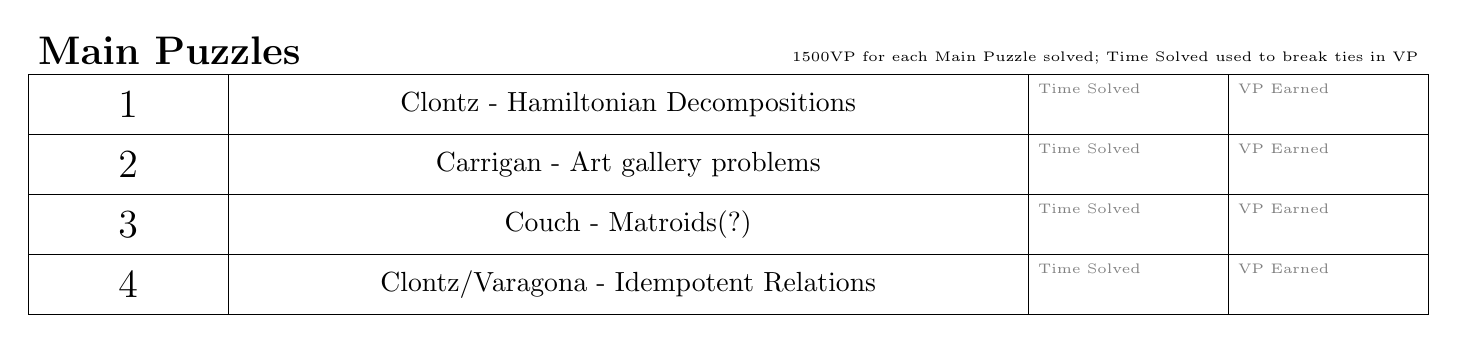
\begin{tikzpicture}[x=1in,y=-0.3in]
  \node[anchor=south west] at (0,0) {\Large\textbf{Main Puzzles}};
  \draw (0,0) rectangle +(7,1);
  \draw (0,1) rectangle +(7,1);
  \draw (0,2) rectangle +(7,1);
  \draw (0,3) rectangle +(7,1);
  \draw (1,0) -- +(0,4);
  \draw (5,0) -- +(0,4);
  \draw (6,0) -- +(0,4);
  \node at (0.5,0.5) {\Large 1};
  \node at (0.5,1.5) {\Large 2};
  \node at (0.5,2.5) {\Large 3};
  \node at (0.5,3.5) {\Large 4};
  \node at (3,0.5) {Clontz - Hamiltonian Decompositions};
  \node at (3,1.5) {Carrigan - Art gallery problems};
  \node at (3,2.5) {Couch - Matroids(?)};
  \node at (3,3.5) {Clontz/Varagona - Idempotent Relations};
  \node[color=gray,anchor=north west] at (5,0)
    {\tiny Time Solved};
  \node[color=gray,anchor=north west] at (5,1)
    {\tiny Time Solved};
  \node[color=gray,anchor=north west] at (5,2)
    {\tiny Time Solved};
  \node[color=gray,anchor=north west] at (5,3)
    {\tiny Time Solved};
  \node[color=gray,anchor=north west] at (6,0)
    {\tiny VP Earned};
  \node[color=gray,anchor=north west] at (6,1)
    {\tiny VP Earned};
  \node[color=gray,anchor=north west] at (6,2)
    {\tiny VP Earned};
  \node[color=gray,anchor=north west] at (6,3)
    {\tiny VP Earned};
  \node[anchor=south east] at (7,0)
    {\tiny 1500VP for each Main Puzzle solved;
    Time Solved used to break ties in VP};
\end{tikzpicture}

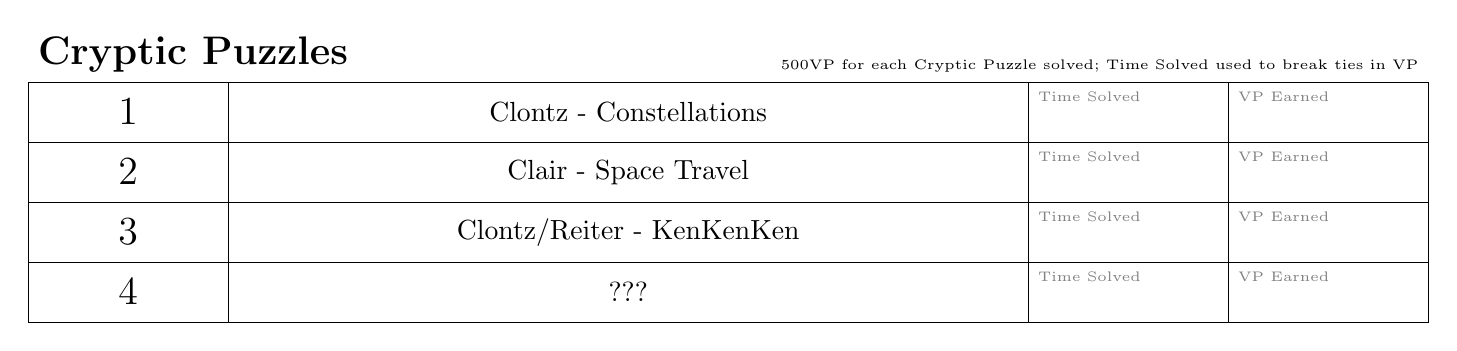
\begin{tikzpicture}[x=1in,y=-0.3in]
  \node[anchor=south west] at (0,0) {\Large\textbf{Cryptic Puzzles}};
  \draw (0,0) rectangle +(7,1);
  \draw (0,1) rectangle +(7,1);
  \draw (0,2) rectangle +(7,1);
  \draw (0,3) rectangle +(7,1);
  \draw (1,0) -- +(0,4);
  \draw (5,0) -- +(0,4);
  \draw (6,0) -- +(0,4);
  \node at (0.5,0.5) {\Large 1};
  \node at (0.5,1.5) {\Large 2};
  \node at (0.5,2.5) {\Large 3};
  \node at (0.5,3.5) {\Large 4};
  \node at (3,0.5) {Clontz - Constellations};
  \node at (3,1.5) {Clair - Space Travel};
  \node at (3,2.5) {Clontz/Reiter - KenKenKen};
  \node at (3,3.5) {???};
  \node[color=gray,anchor=north west] at (5,0)
    {\tiny Time Solved};
  \node[color=gray,anchor=north west] at (5,1)
    {\tiny Time Solved};
  \node[color=gray,anchor=north west] at (5,2)
    {\tiny Time Solved};
  \node[color=gray,anchor=north west] at (5,3)
    {\tiny Time Solved};
  \node[color=gray,anchor=north west] at (6,0)
    {\tiny VP Earned};
  \node[color=gray,anchor=north west] at (6,1)
    {\tiny VP Earned};
  \node[color=gray,anchor=north west] at (6,2)
    {\tiny VP Earned};
  \node[color=gray,anchor=north west] at (6,3)
    {\tiny VP Earned};
  \node[anchor=south east] at (7,0)
    {\tiny 500VP for each Cryptic Puzzle solved;
    Time Solved used to break ties in VP};
\end{tikzpicture}


\begin{tikzpicture}[x=1in,y=-0.3in]
  \node[anchor=south west] at (0,0) {\Large\textbf{Bonus Puzzle}};
  \draw (0,0) rectangle +(5,1);
  \draw (2,0) -- +(0,1);
  \draw (3,0) -- +(0,1);
  \draw (4,0) -- +(0,1);
  \draw (6,0) rectangle +(1,1);
  \node at (1,0.5) {Holshouser - Origami};
  \node[color=gray,anchor=north west] at (2,0)
    {\tiny First Submission};
  \node[color=gray,anchor=north west] at (3,0)
    {\tiny Second Submission};
  \node[color=gray,anchor=north west] at (4,0)
    {\tiny Third Submission};
  \node[color=gray,anchor=north west] at (6,0)
    {\tiny VP Earned};
  \node[anchor=south east] at (7,0)
    {\tiny Up to 500VP for best submission};
\end{tikzpicture}

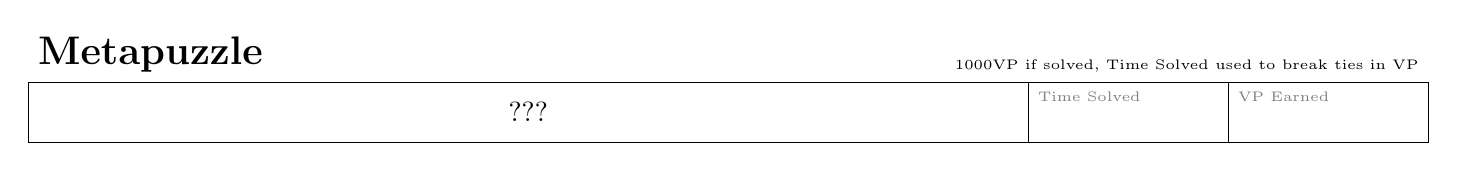
\begin{tikzpicture}[x=1in,y=-0.3in]
  \node[anchor=south west] at (0,0) {\Large\textbf{Metapuzzle}};
  \draw (0,0) rectangle +(7,1);
  \draw (5,0) -- +(0,1);
  \draw (6,0) -- +(0,1);
  \node at (2.5,0.5) {???};
  \node[color=gray,anchor=north west] at (5,0)
    {\tiny Time Solved};
  \node[color=gray,anchor=north west] at (6,0)
    {\tiny VP Earned};
  \node[anchor=south east] at (7,0)
    {\tiny 1000VP if solved,
    Time Solved used to break ties in VP};
\end{tikzpicture}


\begin{tikzpicture}[x=1in,y=-0.3in]
  \fill[color=white] (0,0) rectangle +(7,1);
  \draw (5,0) rectangle +(2,1);
  \draw (6,0) -- +(0,1);
  \node[color=gray,anchor=north west] at (5,0)
    {\tiny Time Acquired};
  \node[color=gray,anchor=north west] at (6,0)
    {\tiny VP Earned};
  \node[anchor=south east] at (7,0)
    {\tiny Up to 500VP if earned,
    Time Acquired used to break ties in VP};
  \node[anchor=east] at (5,0.5) {\small Additional VP};
\end{tikzpicture}


\begin{tikzpicture}[x=1in,y=-0.3in]
  \fill[color=white] (0,0) rectangle +(7,1);
  \draw (6,0) rectangle +(1,1);
  \node[anchor=east] at (6,0.5) {\Large\textbf{Total VP Earned}};
  \node[anchor=south east] at (7,0)
    {\tiny 10,000VP Maximum};
\end{tikzpicture}

%
% \vspace{1em}
%
% {\noindent\LARGE Team Number: \underline{\hspace{0.5in}}
% School Name: \underline{\hspace{3in}}}


%%% Local Variables:
%%% mode: latex
%%% TeX-master: "../mapp-hsc17-game-book"
%%% End:
